\begin{figure}[b]
    \centering
    \begin{subfigure}{0.32\textwidth}
        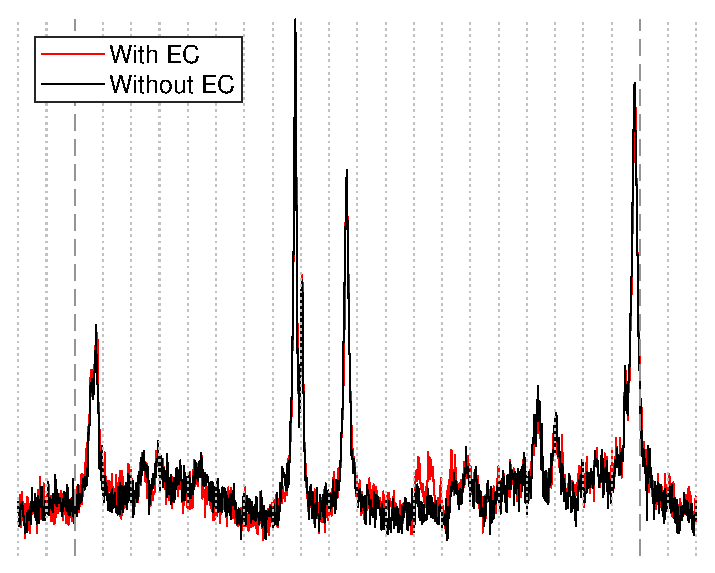
\includegraphics[width=0.95\textwidth, keepaspectratio]{images/eddy/ec=1.eps}
        \caption{Eddy current amplitude = 1.0}
        \label{subfig:ec=1}        
    \end{subfigure}
    \begin{subfigure}{0.32\textwidth}
        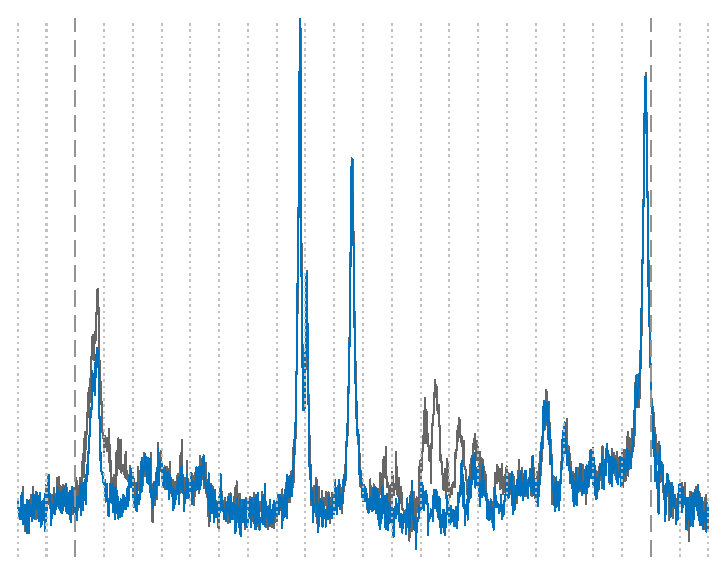
\includegraphics[width=0.95\textwidth, keepaspectratio]{images/eddy/ec=3.eps}
        \caption{Eddy current amplitude = 3.0}
        \label{subfig:ec=3}        
    \end{subfigure}
    \begin{subfigure}{0.32\textwidth}
        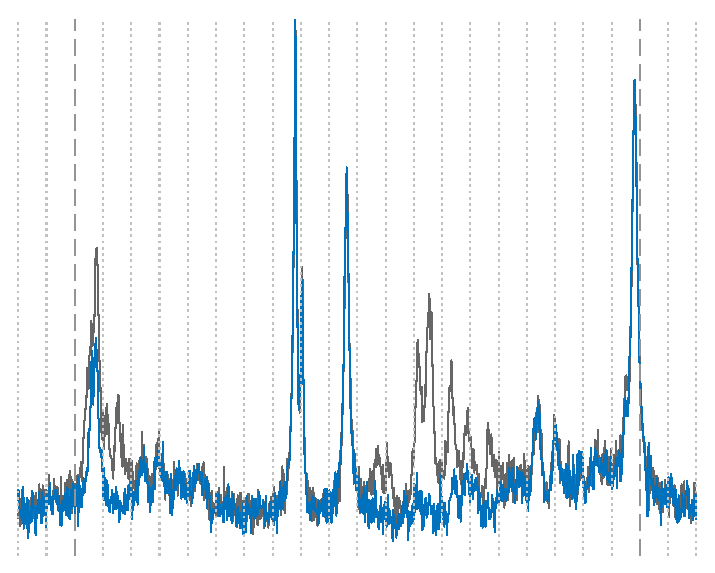
\includegraphics[width=0.95\textwidth, keepaspectratio]{images/eddy/ec=5.eps}
        \caption{Eddy current amplitude = 5.0}
        \label{subfig:ec=5}        
    \end{subfigure}
    \caption{These 3 samples show the effect of eddy currents on MRS spectra to various degrees. The strength of the eddy currents increases from \ref{subfig:ec=1} to \ref{subfig:ec=5}. If the time constant, $tc$, is set too long, the eddy current artifact will appear as a global frequency shift. In these examples, it can be seen that only some frequencies are affected.}
    \label{fig:eddy currents}
\end{figure}
